\documentclass[11 pt]{article}

\usepackage[utf8]{inputenc}
\usepackage[T1]{fontenc}

\usepackage{amsmath}
\usepackage{empheq}
\usepackage{tikz}
\usepackage{tikz-qtree}
\usepackage{listings}
\usepackage{graphicx}
\usepackage{hyperref}
\hypersetup{
  colorlinks,
  citecolor=black,
  filecolor=black,
  linkcolor=blue,
  urlcolor=blue
}

\usepackage{booktabs}
\usepackage[scale=2]{ccicons}
\usepackage{appendix}
% \usepackage[left=2cm,right=2cm,top=1.5cm,bottom=1.5cm]{geometry}
\usepackage[accepted]{icml2017}
\usepackage[french]{babel}

\pagenumbering{roman}


\icmltitlerunning{Rapport de projet ISI-10: AdaNet, Adaptive Neural Newtorks.}

\begin{document}

\twocolumn[
\icmltitle{Rapport de projet ISI-10:\\ AdaNet, Adaptive Neural Newtorks.}

\begin{icmlauthorlist}
  \icmlauthor{Luc Blassel \href{mailto:luc.blassel@agroparistech.fr}{luc.blassel@agroparistech.fr}}{equal}
  \icmlauthor{Romain Gautron \href{mailto:romain.gautron@agroparistech.fr}{romain.gautron@agroparistech.fr}}{equal}
\end{icmlauthorlist}
\vskip 0.3in
]

\section*{Introduction}
\paragraph{}Le but de ce projet est de reproduire les expériences et les méthodes issues du papier suivant :\\
\href{https://arxiv.org/pdf/1607.01097.pdf}{C. Cortes, X. Gonzalvo, V. Kuznetsov, M. Mohri, S. Yang \emph{AdaNet: Adaptive Structural Learning of Artificial Neural Networks}}.
En essayant de reproduire leur méthode qui consiste à construire des réseaux de neurones dont la structure est apprise et optimisée en même temps que les poids. Cette méthode sera appliquée sur une tache de classification binaire issue du jeu de données d'images CIFAR-10.

\section{Comment marche AdaNet?}
\paragraph{}La structure du réseau est générée. Le réseau entier qu'on appellera le réseau AdaNet, est augment\'e à chaque itération par un sous réseau. Ce sous réseau est choisi en fonction de son effet sur une fonction objectif pour pouvoir sélectionner le meilleur sous réseau à rajouter au réseau Adanet à chaque étape. Pour bien comprendre le déroulement de ce processus on notera: $f_t$ le réseau AdaNet a l'étape $t$, $h_t$ et $h'_t$ les sous réseaux candidats (a l'étape $t$) avec pour chacun de ces sous réseaux $h_{t,k}$ la $k^{eme}$ couche du sous réseau et $h_{t,k,j}$ le $j_{eme}$ neurone de cette couche. $l$ est le nombre de couche maximale du sous réseau.
\paragraph{}L'algorithme se déroule alors selon ces étapes:
\begin{enumerate}
	\item \textbf{Initialisation du réseau: }On commence par générer les couches d'entrée et de sortie.
	\item \textbf{Génération de sous-réseaux candidats: }On génère deux sous réseaux candidats\emph{(cf. Figure \ref{candidateModels})}:
	\begin{itemize}
		\item Un qui a une profondeur identique au sous réseau généré précédemment $\rightarrow k$
		\item Un qui augmente la profondeur de 1 par rapport au sous réseau précédent $\rightarrow k+1$
	\end{itemize}
	Ces deux sous réseaux obéissent aux mêmes règles de connectivité. C'est à dire que le première couche du réseau du sous réseau $h_t$  est reliée à la couche d'entrée de $f_t$, la dernière couche $h_{t,l}$ du sous réseau est forcement connectée à la couche de sortie de $f_t$. Pour les couches intermédiaires, chaque couche $h_{t,k}$ est forcement reliée à $h_{t,k-1}$ et peut être reliée aux couches de niveau précédent dans tous les sous réseaux précédemment générés, c'est à dire $h_{t\in[1,t-1],k-1}$.
	\emph{Lors de la première itération il faut forcement choisir le sous réseau qui augmente la profondeur puisque $k=0$}
	\item \textbf{Choix du sous-réseau: }Parmi ces deux sous réseaux candidats $\mathbf{h}$ et $\mathbf{h'}$ on choisit celui qui, après un entraînement, minimise le plus la fonction objectif suivante:
	\begin{multline*}
		F_t(\mathbf{w,h}) = \frac{1}{m}\sum^m_{i=1}\Phi(1-y_if_{t-1}(x_i)-y_i\mathbf{w\cdot h}(x_i)) \\
        + \mathcal{R}(\mathbf{w,h})
	\end{multline*}
	Avec $x_i$ les exemples d'entraînement, $y_i$ les réponses attendues, $m$ Le nombre d'exemples,$\mathbf{w}$ Les poids associ\'es au sous réseau candidat $\mathbf{h}$ et $\Phi$ une fonction (soit la fonction exponentielle soit la fonction logistique). Le terme $\mathcal{R}(\mathbf{w,h})$ est un terme de régularisation qui est laiss\'e à $0$ lors des expérimentations.\\
	Si $F(\mathbf{w,h})>F(\mathbf{w,h'})$ alors le sous réseau candidat $\mathbf{h'}$ est choisi et $\mathbf{h}_t \leftarrow \mathbf{h'}$\\
	\item \textbf{Condition d'arrêt: }Une fois que le meilleur sous réseau est sélectionn\'e on regarde si celui ci a apporté une amélioration au réseau AdaNet. Si la fonction objectif de l'entraînement de $f_{t-1}$ \emph{(qui n'est pas le même que celle utilisée pour le choix du meilleur sous réseau)} est meilleure avec le sous réseau que sans alors: $f_t \leftarrow f_{t-1}+\mathbf{w}^*\mathbf(h)_t$ sinon l'intégration du sous réseau n'apporte rien de plus au réseau $f_{t-1}$ et celui est retourn\'e, terminant alors l'exécution de l'algorithme. Si cette condition d'arrêt n'est jamais vérifiée, l'algorithme s'arrête au bout de $T$ itérations et retourne le réseau $f_T$
\end{enumerate}
\paragraph{}On voit donc bien que la génération et l'ajustement des poids du réseau se fait itérativement à chaque étape.\\ \bigskip
\begin{figure}[h]
	\centering
	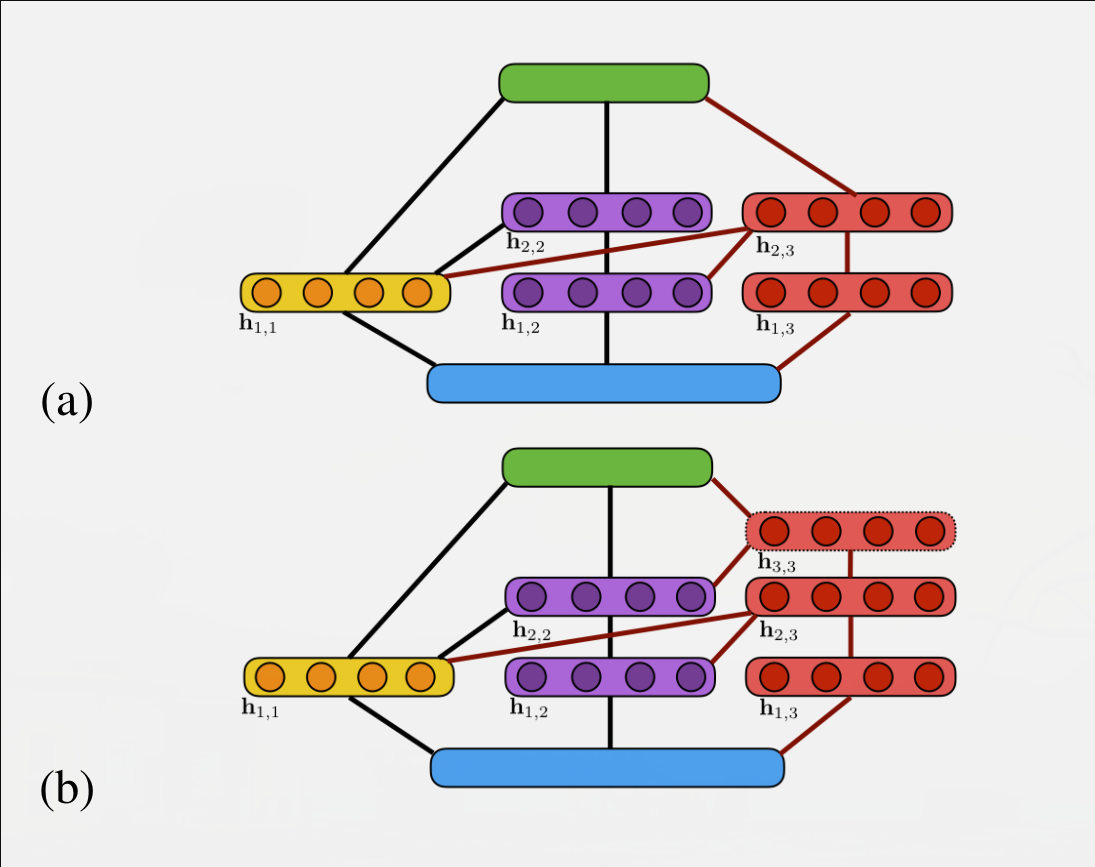
\includegraphics[width=0.5\textwidth]{schema.png}
	\caption{Les deux sous réseaux candidats générés à l'étape $3$ (en rouge), un de profondeur $k=2$ comme le sous réseau choisi à l'étape précédente (en bleu), et un de profondeur $k=3$ qui augmente la profondeur générale de $1$. Ce sont ces deux réseaux AdaNets potentiels qui vont être évalués}
	\label{candidateModels}
\end{figure}

\section{Choix lors des expérimentations}
\subsection{Choix du dataset}

	Une parmi deux expérimentations à reproduire était au choix : 
	\begin{itemize}
		\item CIFAR-10 dataset
		\item Criteo dataset
	\end{itemize}

	Le choix s'est porté sur la taille du jeu de données à traiter. Si l'on ne retient que deux classes à traiter, CIFAR contient moins de 10000 éléments par classe tandis que le dataset Criteo contient 30 millions de lignes pour le set d'entraînement.

\subsection{Choix du langage et de l'API}
	On programme sous \texttt{Python} et on utilise l'API \texttt{Keras} pour sa syntaxe simple et sa très grande modularité. Le backend utilisé est \texttt{Tensorflow} mais cela n'a aucune influence sur le code dans \texttt{Keras}.

\subsection{Imprécisions du papier}

\subsubsection{Gestion des tenseurs multiples en entrée}
\label{subsec:mult}
On ne sait pas si lorsqu'une couche reçoit les entrées de plus d'une autre couche les tenseurs sont soit :
\begin{itemize}
	\item juxtaposés (fonction \texttt{concatenate})
	\item sommés (fonction \texttt{add})
\end{itemize}

\subsubsection{Régularisation des sous réseaux}
On ne sait pas explicitement si les sous réseaux sont régularisés à l'aide d'une norme $L_{1}$ ou $L_{2}$. L'utilisation du terme $\lambda$ nous fait choisir la norme $L_{1}$. On ne sait pas non plus si c'est la loss qui est régularisée ou les poids lors de l'apprentissage. On choisit de régulariser avec une norme $L_{1}$ les poids de chaque couche des sous réseaux ainsi que la couche de sortie.

\section{Choix pour l'implémentation}
\subsection{Traitement des données en entrée}
Pour traiter les images en dehors d'un réseau de convolution, on vectorise celles-ci en un vecteur de longueur $width*height*3$

\subsection{Architecture des couches d'entrée et de sortie}
\begin{itemize}
	\item La couche d'entrée est de taille $width*height*3$ soit 3072 pour les images de CIFAR-10
	\item La couche de sortie contient un unique neurone et une activation sigmoïde, la classification étant binaire
\end{itemize}

\subsection{Génération des sous réseaux}
Nous choisissons de générer les sous réseaux aléatoirement. Chaque couche est connectée à la précédente du même sous réseau, mais les connexions avec les couches de niveau inférieur des autres sous réseaux est aléatoire. 

\subsection{Choix de la fonction objectif}

Nous choisissons de générer les sous réseaux aléatoirement. Chaque couche est connectée à la précédente du même sous réseau, mais les connexions avec les couches de niveau inférieur des autres sous réseaux est aléatoire. 

\subsection{Fonction objectif}
\label{subsec:fobj}
\begin{multline*}
F_t(\mathbf{w,h})=\frac{1}{m}\sum^m_{i=1}\Phi(1-y_if_{t-1}(x_i)-y_i\mathbf{w\cdot h}(x_i))\\
+ \mathcal{R}(\mathbf{w,h})
\end{multline*}
Avec $x_i$ les exemples d'entraînement, $y_i$ les réponses attendues, $m$ le nombre d'exemples,$\mathbf{w}$ les poids associés au sous réseau candidat $\mathbf{h}$ et $\Phi$ la fonction exponentielle. Le terme $\mathcal{R}(\mathbf{w,h})$ est un terme de régularisation qui est laiss\'e à $0$ lors des expérimentations.

\bigskip

On interprète cette formule avec les conditions ci-dessus comme :
\begin{multline*}
F_t(\mathbf{h})=\\
\frac{1}{m}\sum^m_{i=1}\exp(1-y_i \cdot pred_{t-1}(x_i)-y_i \cdot pred_{t-1 + \mathbf{h}}(x_i))
\end{multline*}

\section{Implémentation pratique}
\paragraph{}Nous avons tenté d’être le plus fidèle possible à l’implémentation du papier. Nous avons du prendre quelques décisions cependant lorsque le papier n’était pas explicite sur la méthode utilisée.
\subsection{Génération et sélection des sous réseaux}
\paragraph{}Nous fournissons un paramètre à l'algorithme qui permet de spécifier combien de sous modèles candidats sont générés \`a chaque itération avec un paramètre \emph{reps}. Étant donne que dans le papier il n'y a que deux types de sous-réseaux générés (même profondeur ou profondeur +1) nous avons fait le choix de générer des sous réseaux de même profondeur que le réseau du pas de temps précédent pour les $\frac{reps}{2}$ premières itérations et des sous réseaux plus profonds pour les itérations suivantes.
\paragraph{}Les connexions entre les différentes couches suivent les règles de connectivité décrites plus haut, c'est \`a dire dernière couche du sous réseau reliée à la couche de sortie, première couche du sous réseau reliée à la couche d’entrée et toutes les couches internes sont reliées entre-elles au sein d'un même sous réseau. La variabilité entre les sous réseaux candidats apparaît dans la connectivité entre les sous réseaux candidats. Pour chaque couche du sous-réseau candidat considéré, un nombre aléatoire de connexions aux sous couches de profondeur inférieure de 1 parmi les sous réseaux générés aux pas de temps précédents, est sélectionné.

\paragraph{}Le nombre de neurones par sous couche des sous-réseaux candidats est déterminé par un paramètre fix\'e au début de l'algorithme. Donc toute la variabilité entre les candidats vient du nombre de connexions aux sous-réseaux précédents et au changement de profondeur.

\paragraph{}Tous les sous-réseaux candidats sont insérés dans le réseau adanet de l’étape précédente pour être évalués, après entraînement, sur un set de test, selon la fonction objective définie en \ref{subsec:fobj}. Le résultat de la fonction objective le plus bas est mis en mémoire ainsi que le modèle adanet correspondant, et mis à jour si besoin à chaque évaluation de candidat. A la fin de l’évaluation des candidats le meilleur réseau est sauvegard\'e sur le disque et utilise comme modèle de base pour l’étape suivante.

\subsection{Implémentation de la gestion d’entrées multiples}
\paragraph{}Comme dit dans la partie \ref{subsec:mult}, il n'est pas dit dans le papier, comment la gestion du nombre de neurones entrant variable pour certaines couches. Si on concatène les tenseur des couches entrantes on change la taille d’entrée de la couche supérieure. Ceci pose un problème lors du chargement des poids du modèle adanet de l’étape précédente 
puisque le tenseur de poids sauvegardes et le nouveau tenseur ne font plus la même taille. Une solution que nous avons utilisée est de ne pas charger les poids précédents pour ces couches de concaténation. cependant cela peut faire perdre en performance. Nous avons donc préféré sommer les tenseurs entrants et garder les poids de l’itération précédente. 

\subsection{Problème de flexibilité}
\paragraph{} Puisque la structure change constamment au fur et à mesure des itérations on ne peut pas se contenter de sauvegarder les modèles directement au disque puisque l'on ne peut pas changer les modèles une fois qu'ils sont compil\'es. Pour pouvoir passer outre ce problème nous avons sauvegard\'e la structure exacte du modèle dans un dictionnaire et on reconstruit le modèle \`a partir de ce dictionnaire à chaque itération. Une fois construit on charge les poids de l'ancien modèle dans les couches qu'il a en commun avec le nouveau à chaque itération le dictionnaire correspondant au meilleur modèle est simplement s\'erialisable puisque ça n'est que du texte. 

\subsection{Condition d’arrêt}
\paragraph{}Dans le papier il est dit que l'algorithme s’arrête lorsque l'ajout d'un nouveau sous-réseau ne fait pas diminuer sa fonction objectif. Au regard de nos puissances limitées de calcul nous avons fait le choix de s’arrêter lorsque la diminution de la fonction objective passe sous un certain seuil. L’entraînement des différents sous-réseaux est aussi soumis à une condition similaire d’arrêt lorsque l'erreur de classification sur un jeu de validation ne diminue plus. 

\section{Résultats}
\paragraph{}Nous n'avons pas pu refaire toutes les optimisations d'hyper-paramètres qui ont été faites dans le papier, donc nous avons simplement choisi un jeu d'hyper-paramètres pour nos expérimentations:
\begin{itemize}
  \item $n = 150$, le nombre de neurones dans chaque couche
  \item $\lambda = 0.000001$, le paramètre de normalisation
  \item $\eta = .001$, le taux d'apprentissage
  \item $T = 10$, le nombre de répétitions
  \item $reps = 5$ le nombre de sous-réseaux générés a chaque étape
\end{itemize}
\paragraph{}Nous avons ensuite exécuté notre algorithme sur différents jeux de données binaires (les mêmes que ceux du papier), mesur\'e leur précision de classification sur un jeu de test et sur 10 exécutions pour avoir une performance moyenne et un écart-type. Il est à noter que le set CIFAR-10 est déjà séparé en un set de test et d'entraînement. On obtient alors les résultats de la table \ref{table:res}
\paragraph{} Les résultats sont très variables en fonction des couples. Cela s'explique par le fait qu'aucune optimisation des hyper-paramètres n'a été faite. Ainsi, à la faveur des choix arbitraires que l'on a fait on peut se retrouver tant avec de très bon résultats (deer-horse) qu'avec de mauvais résultats.
\begin{table*}[t]
  \centering
    \begin{tabular}{c c c}
      	\toprule
       	 jeu de données &résultat de notre version &résultat papier \\
        \midrule
      	\texttt{deer-truck} & $\mathbf{0.2741\pm0.0391}$ & $0.9372 \pm 0.0082$ \\
      	\texttt{deer-horse} & $\mathbf{0.8731 \pm0.0097}$ & $0.8430 \pm 0.0076$ \\
      	\texttt{automobile-truck} & $\mathbf{0.2521 \pm0.0204}$ & $0.8461 \pm 0.0069$\\
        \texttt{cat-dog} & $\mathbf{ 0.3085\pm0.0449}$ & $0.6924 \pm 0.0129$\\
        \texttt{dog-horse} & $\mathbf{0.5711 \pm0.0172}$ & $0.8350 \pm 0.0089$\\
      	\bottomrule
    \end{tabular}
    \caption{Comparaison des précisions de classification entre la version du papier et la notre}
    \label{table:res}
\end{table*}


\section{Conclusion}
Nous avons essayé dans ce projet de reproduire les résultats d'Adanet. Nous avons été contraints de faire des choix, notamment sur la génération des sous réseaux et nous avons du nous priver d'optimisation des hyper-paramètre (nécessité d'implémenter en plus une méthode sophistiquée). De ce fait, les résultats que nous avons obtenus sont, exception faite pour deer-horse, nettement moins bons que ceux obtenus dans le papier. Certains des résultats que nous avons obtenus (deer-truck, automobile-truck et cat-dog) semblent biais\'es puisque l’on obtient des précisions inférieures a $50\%$.  
Dans tous les cas, des performances nettement meilleures que celles obtenues dans le papier peuvent être obtenues via du transfert learning (précision supérieure à 90\%). Ceci ne montre pas clairement l'intérêt de cette méthode très nécessiteuse de calculs (génération d'un grand nombre de sous réseaux). Cependant, si l'on ne dispose pas d'un modèle entraîné pour faire de l'apprentissage par transfert, alors cette approche peut être intéressante.

\end{document}
